This chapter describes the dataset that KickSense was built on and reports the results obtained from it. It opens with the composition and characteristics of the corpus, including the properties that make it difficult, then presents the qualitative evaluation, which examines whether the pose extraction is visually faithful and where it fails, and then the quantitative evaluation, which reports the metrics obtained on a held out test split that was never used for model selection. The chapter closes with the ablation study, the development history across all recorded runs, and a comparison of the evaluation protocol against that of the base paper. Every number quoted here is computed by the scripts in \texttt{report\_assets} from the artefacts in the repository, and every figure was generated by the same run that produced the numbers.

\section{Which Dataset Is Used}

No public dataset annotates the direction of a football penalty kick, as established in Chapter 2, so the corpus used here was collected and annotated specifically for this project. It has two distinct components, and the difference between them turns out to be one of the most informative findings in the whole evaluation.

The first component is broadcast footage. Penalties were sourced from recorded matches across seventeen competitions, including the men's World Cup 2022, the Women's World Cup 2023, AFCON 2025, the Leagues Cup 2023, the Champions League 2008, Euro 2020, Euro 2024 and the FA Cup 2022, and each source match was cut into individual single penalty clips. This component provides breadth of players, stadiums and techniques, and it is the only realistic way to obtain elite level penalties at volume.

The second component is footage recorded specifically for this project. Sixty one clips were captured during dedicated local sessions, framed so that the kicker occupies a substantial part of the image and is not occluded. This component was added to increase the size of the corpus, but its more important contribution is that it provides the camera framing that broadcast footage does not, which as Section 4.5 shows is the single largest determinant of whether pose estimation succeeds at all.

\section{Dataset Insights}

\subsection{Media Type, Volume and Acquisition Properties}

The dataset is video rather than still imagery, which is essential rather than incidental. A single frame of a penalty run up cannot distinguish a player who is about to open the hips from a player who is about to close them, because the discriminative information is in how the body configuration changes over time rather than in any one configuration. Every clip must therefore be treated as a temporal sequence, and the modelling problem is sequence classification rather than image classification.

\renewcommand{\arraystretch}{1.25}
\small
\begin{longtable}{|>{\bfseries}p{6.4cm}|p{7.4cm}|}
\hline
\textbf{Property} & \textbf{Value} \\ \hline
\endfirsthead
\hline
\textbf{Property} & \textbf{Value} \\ \hline
\endhead
\hline
\multicolumn{2}{r}{\textit{Continued on next page}} \\
\hline
\endfoot
\hline
\endlastfoot
Media type & Video, single camera, no depth channel \\ \hline
Video files collected & 301 \\ \hline
Clips with complete annotation & 259 \\ \hline
Clips with a saved keypoint array & 257 \\ \hline
Sequences usable after the quality gate & 225 \\ \hline
Resolutions present & 1280 by 720 (164 files), 640 by 360 (137 files) \\ \hline
Frame rates present & 25 fps (184 files), 30 fps (109 files), 50 fps (8 files) \\ \hline
Colour format & 3 channel RGB, no depth or infrared \\ \hline
Extracted frames per clip, mean & 161 \\ \hline
Extracted frames per clip, median & 161 \\ \hline
Extracted frames per clip, range & 1 to 2,495 \\ \hline
Total frames extracted across the corpus & 41,476 \\ \hline
Total frames in which a pose was detected & 25,167 \\ \hline
Total frames actually consumed by the model & 6,526 (15.7 percent of extracted) \\ \hline
Sequence length after resampling & 26 time steps \\ \hline
Features per time step & 132 (33 landmarks by 4 values) \\ \hline
Model input tensor shape & (26, 132) \\ \hline
Direction label counts & Left 107, Right 94, Center 58 \\ \hline
Outcome label counts & Goal 225, Saved 21, Missed 13 \\ \hline
Ball placement label counts & Top left 104, Center 85, Top right 60, Bottom right 6, Bottom left 3 \\ \hline
Dominant foot label counts & Right 253, Left 6 \\ \hline
Shot power scale & Integer 1 to 10, manually annotated \\ \hline
Distinct source competitions & 17 \\ \hline
Distinct players & 138 \\ \hline
Train / validation / test split & 157 / 34 / 34 sequences \\ \hline
\caption{Summary of the KickSense dataset and its acquisition properties}
\label{tab:dataset-summary}
\end{longtable}
\normalsize

\noindent
\textbf{Description:} This table gives the complete numerical description of the corpus in one place. Three rows deserve particular attention. The gap between 259 annotated clips and 225 usable sequences is the cost of the pose quality gate and is quantified in Section 4.5. The gap between 41,476 extracted frames and 6,526 consumed frames is the effect of temporal resampling, and it shows that only 15.7 percent of extracted frames reach the model directly, the remainder serving to determine which frames the resampling selects and to establish the detection ratio the quality gate depends on. The dominant foot distribution, at 253 right footed against 6 left footed, is so skewed that the model cannot learn anything foot specific, which is exactly why the mirror augmentation described in Chapter 3 is valuable.

\begin{figure}[H]
    \centering
    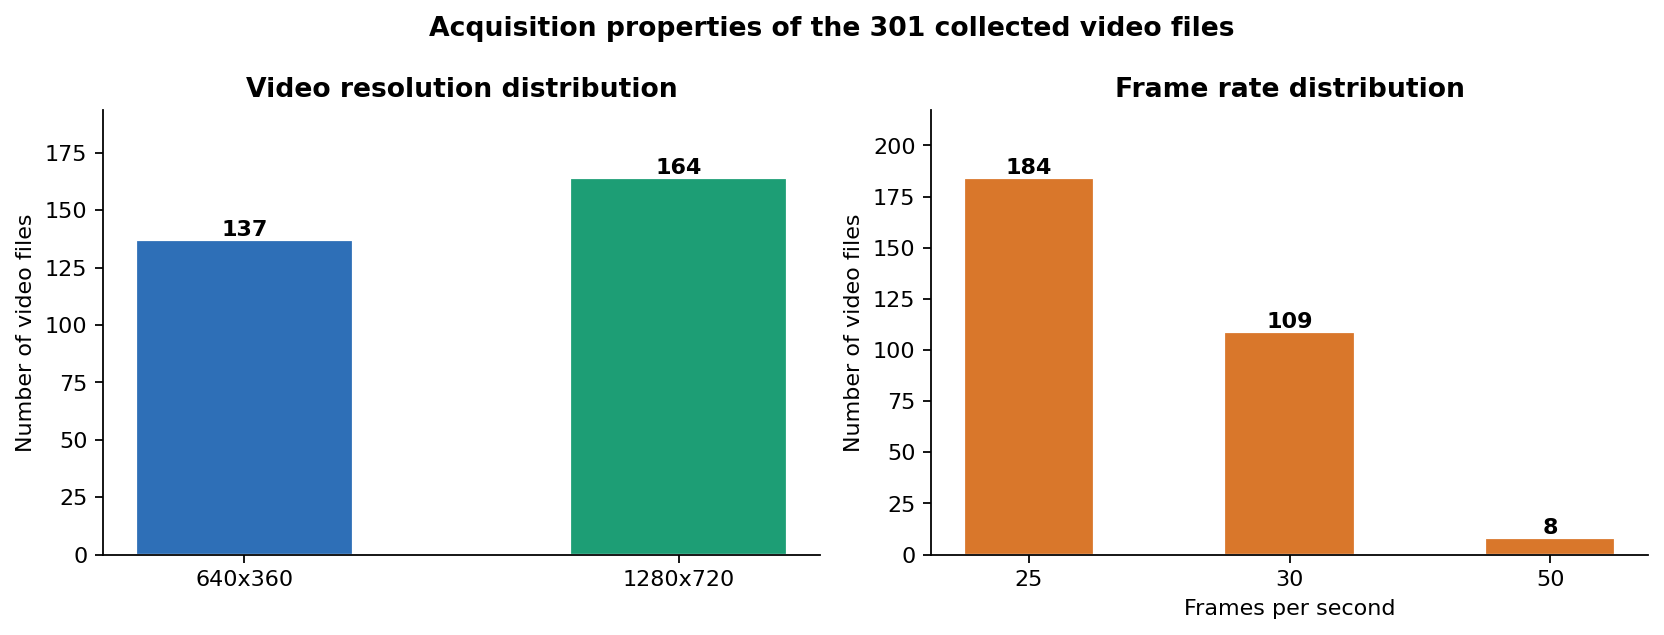
\includegraphics[width=0.99\textwidth]{fig12_resolution_framerate.png}
    \caption{Resolution and frame rate distribution across the 301 collected video files}
    \label{fig:resolution}
\end{figure}

\noindent
\textbf{Description:} The corpus is split between two resolutions and three frame rates, with no single setting dominating. This heterogeneity is the reason the preprocessing stage must normalise coordinates and resample time rather than assuming a fixed acquisition format. Because MediaPipe returns coordinates normalised to the image dimensions, resolution differences are absorbed automatically; frame rate differences are absorbed by the fixed length temporal resampling.

\subsection{Label Distribution}

\begin{figure}[H]
    \centering
    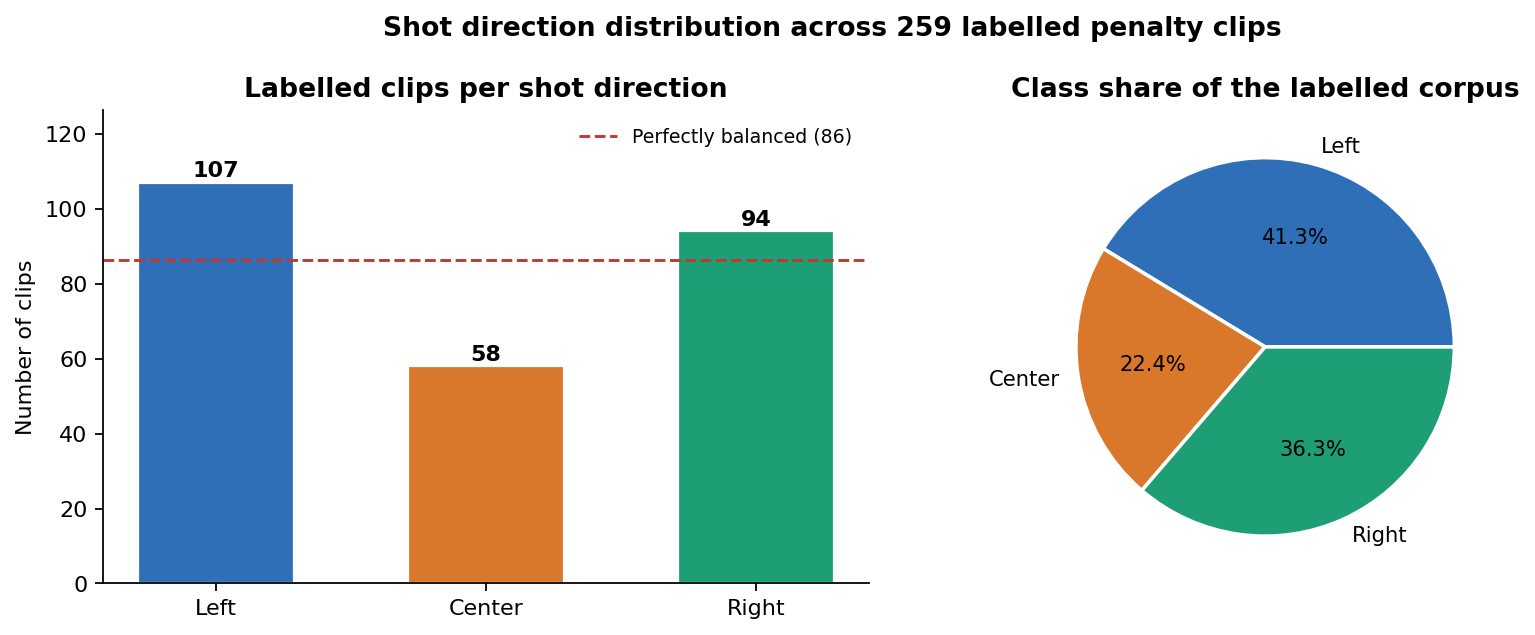
\includegraphics[width=0.99\textwidth]{fig10_class_distribution.png}
    \caption{Shot direction distribution across the 259 labelled penalty clips}
    \label{fig:class-dist}
\end{figure}

\noindent
\textbf{Description:} The three direction classes are unbalanced, with 107 left, 94 right and 58 centre examples against 86 that a perfectly balanced corpus would contain in each class. The imbalance is not an artefact of collection but a property of the sport, because penalty takers aim for the corners far more often than down the middle. The consequence is that the centre class has roughly half the support of the other two, and the per class metrics in Section 4.6 show precisely this effect.

\begin{figure}[H]
    \centering
    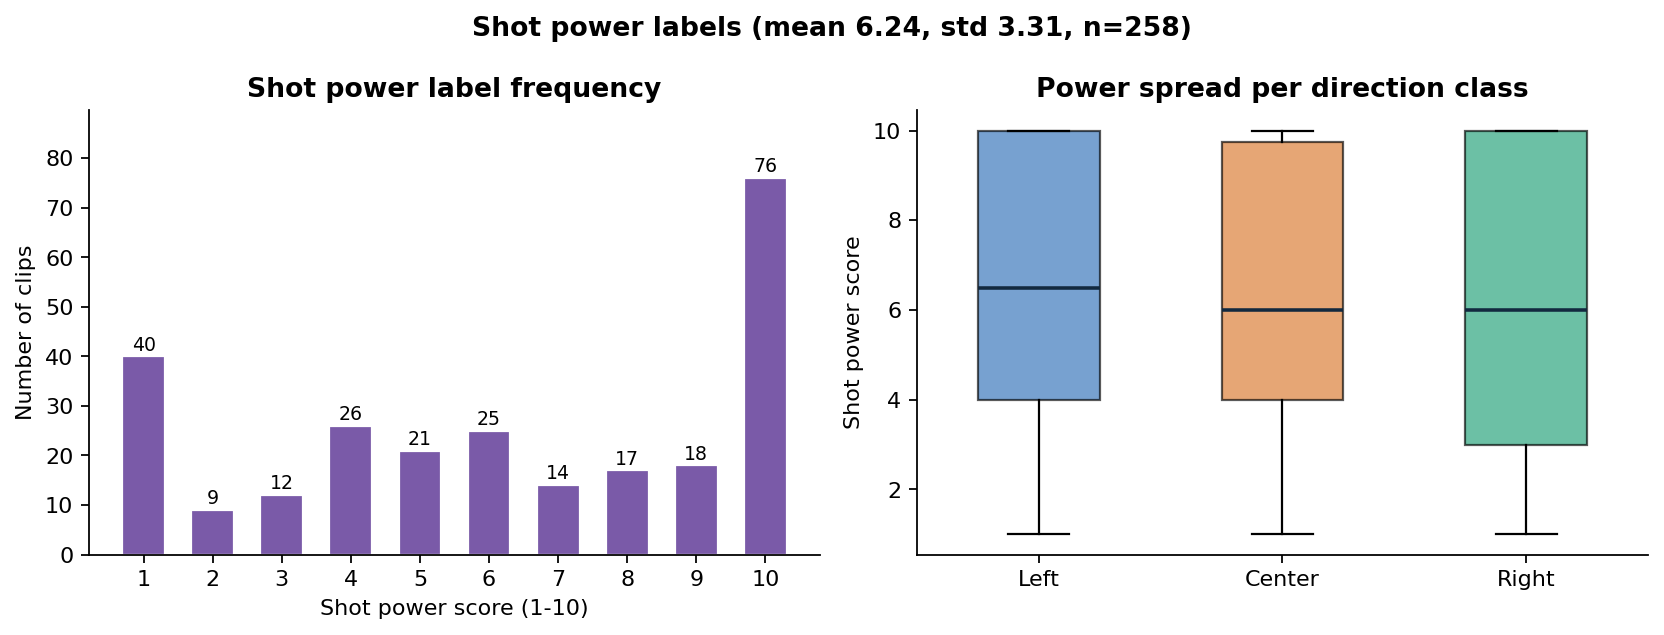
\includegraphics[width=0.99\textwidth]{fig11_power_distribution.png}
    \caption{Shot power label frequency and its spread within each direction class}
    \label{fig:power-dist}
\end{figure}

\noindent
\textbf{Description:} The left panel exposes a genuine weakness in the annotation. The power scale is nominally continuous from one to ten, but the observed distribution is strongly bimodal, with 76 clips at the maximum value of ten and 40 at the minimum value of one, which indicates that the annotator was in practice making a coarse categorical judgement rather than a graded one. The right panel shows that power is distributed almost identically across the three direction classes, with means of 6.48 for left, 6.17 for centre and 6.00 for right against standard deviations above 3.2 in every class. This is informative in two ways: it confirms that the direction label and the power label are close to statistically independent, so the multi task setup is not merely predicting the same quantity twice, and it means the power head has to work from motion characteristics alone with no help from the direction signal.

\begin{figure}[H]
    \centering
    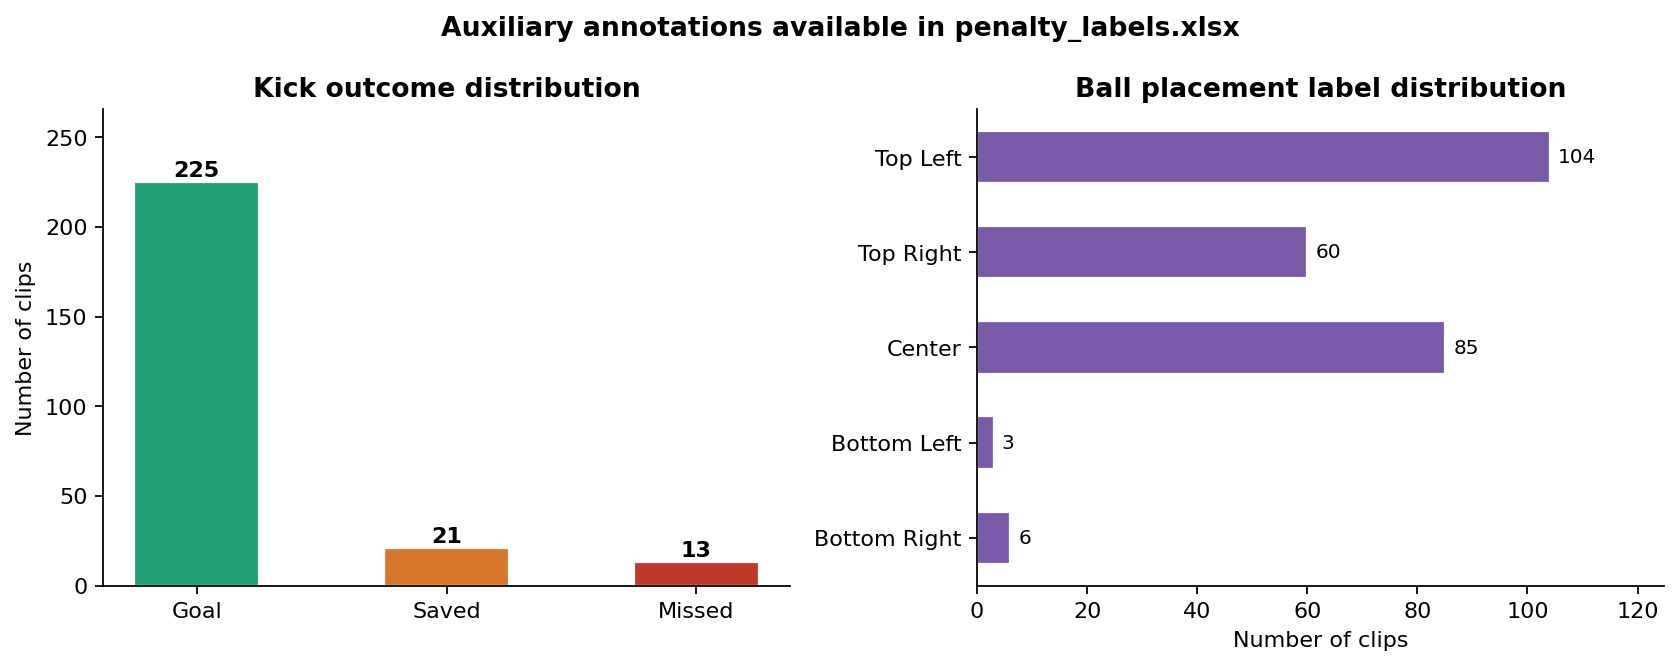
\includegraphics[width=0.99\textwidth]{fig16_outcome_placement.png}
    \caption{Kick outcome and ball placement annotations available in the label file}
    \label{fig:outcome}
\end{figure}

\noindent
\textbf{Description:} These two auxiliary annotations are present in the label file but are not currently consumed by the model. The outcome distribution is extremely skewed, with 225 goals against 21 saves and 13 misses, which reflects the fact that most penalties at elite level are scored and which makes outcome unusable as a prediction target at this dataset size. Ball placement carries more information, distinguishing five regions of the goal, and integrating it as an auxiliary task is listed as future work in Chapter 5 rather than claimed as a current capability.

\begin{figure}[H]
    \centering
    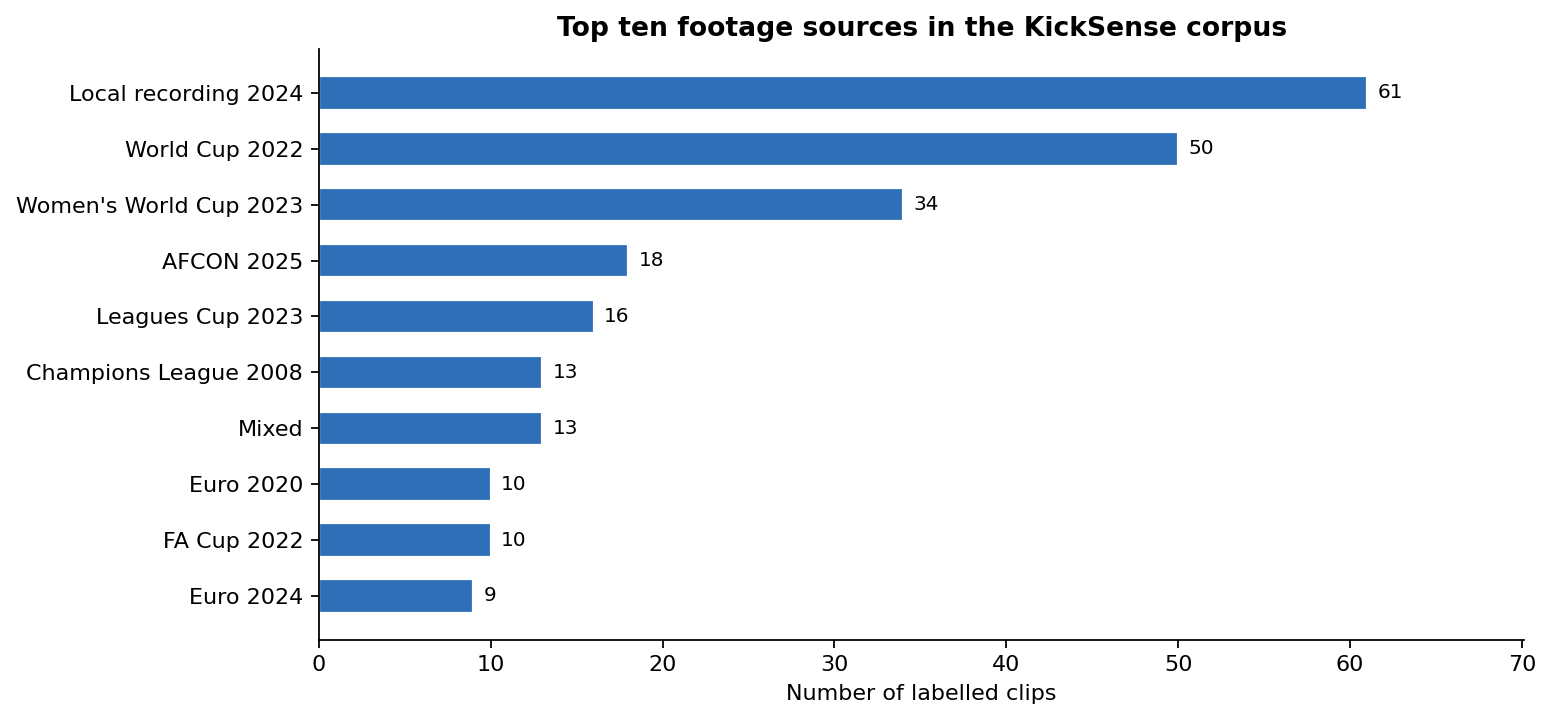
\includegraphics[width=0.92\textwidth]{fig17_source_distribution.png}
    \caption{Composition of the corpus by footage source}
    \label{fig:sources}
\end{figure}

\noindent
\textbf{Description:} The single largest contributor is the locally recorded session at 61 clips, followed by the men's World Cup 2022 at 50 and the Women's World Cup 2023 at 34, with the remainder distributed across fourteen further competitions. The spread across competitions is desirable because it varies players, stadiums, kit and broadcast style, which reduces the chance that the model latches onto a source specific artefact. The prominence of the local recordings is what makes the comparison in Section 4.5 possible.

\subsection{Temporal Footprint}

\begin{figure}[H]
    \centering
    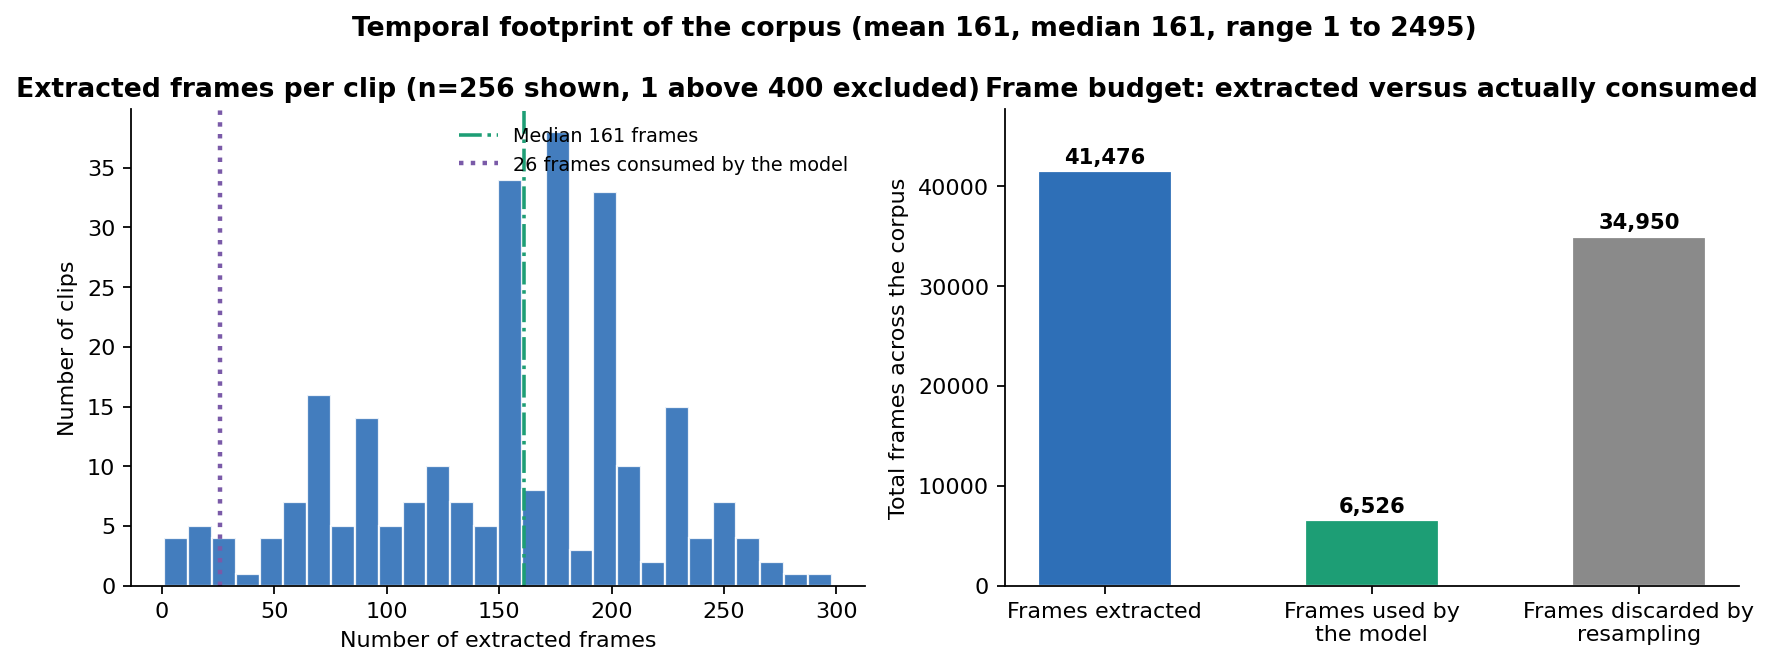
\includegraphics[width=0.99\textwidth]{fig13_frame_count_distribution.png}
    \caption{Frames extracted per clip and the proportion actually consumed by the model}
    \label{fig:frames}
\end{figure}

\noindent
\textbf{Description:} The left panel shows the distribution of extracted frames per clip, which is centred near the median of 161 frames with a long right tail. One clip contains 2,495 frames because the source video was not cut as tightly as the rest, and it is excluded from the histogram to keep the remaining distribution readable. A small number of clips contain fewer than twenty frames and are among those rejected by the quality gate. The right panel quantifies the frame budget explicitly: 41,476 frames were extracted and passed through pose estimation, of which 6,526 reach the model as time steps and 34,950 are discarded by the resampling step. This is the concrete answer to how many frames are extracted against how many are actually used.

\subsection{Feature Space and Normalisation}

The feature space is defined by the landmark topology shown in Figure \ref{fig:landmarks}. Each of the thirty three landmarks contributes four values, giving the one hundred and thirty two features per time step. Landmarks eleven, twelve, twenty three and twenty four additionally serve as the anchors that define the normalisation, since the hip midpoint provides the origin and the shoulder to hip distance provides the unit of length. This has a practical consequence for the dataset: a failure to detect the torso is far more damaging than a failure to detect an extremity, because without the anchors the entire frame cannot be normalised and the frame is lost even if most other landmarks were recovered successfully.

\section{Qualitative Experiments}

The qualitative evaluation asks whether the intermediate representation is visually faithful, in other words whether the skeleton the model receives genuinely corresponds to the player in the video. This matters more here than in a typical classification project, because the model never observes the image, so any systematic failure of the pose stage is invisible in the loss curve and will be silently absorbed as label noise.

\begin{figure}[H]
    \centering
    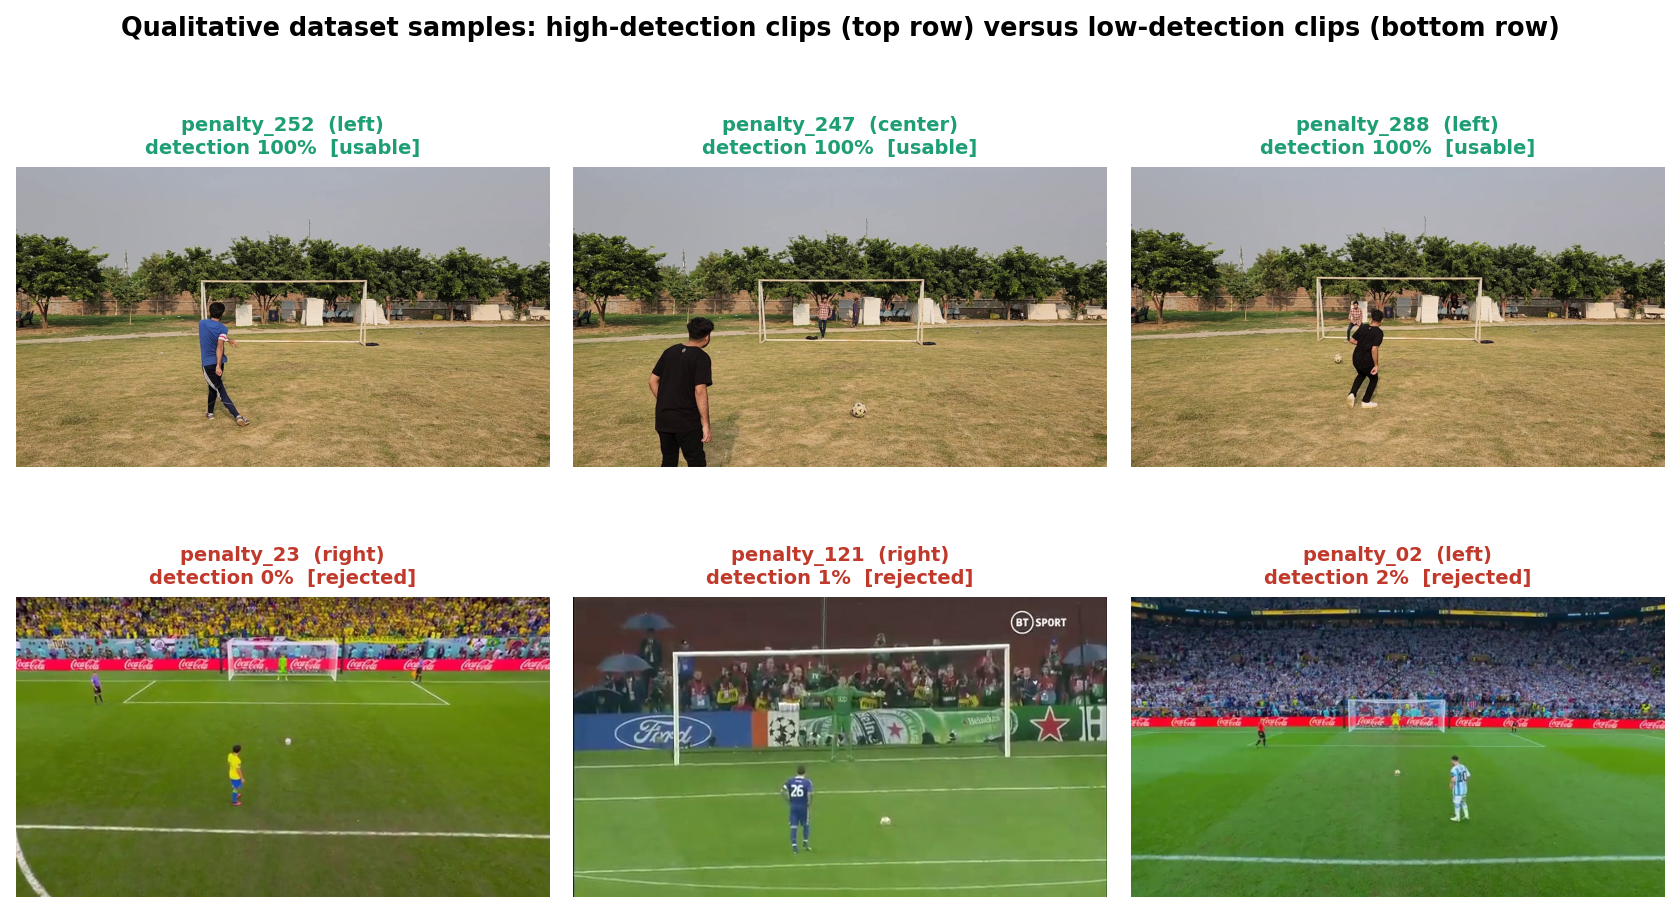
\includegraphics[width=0.99\textwidth]{fig25_qualitative_samples.png}
    \caption{Real frames from the highest and lowest pose detection clips in the corpus}
    \label{fig:qualitative}
\end{figure}

\noindent
\textbf{Description:} This montage is taken directly from the extracted frames and is the most revealing qualitative result in the project. The top row shows the three clips with the highest detection ratios, all at 100 percent, and all three are locally recorded clips in which the kicker occupies a large and unobstructed part of the frame. The bottom row shows the three lowest, at 0, 1 and 2 percent, and all three are broadcast clips filmed from an elevated wide angle in which the kicker occupies a small fraction of the image against a busy crowd background. The failure is therefore not random and not a defect of the pose estimator as such: it is a direct consequence of the subject's apparent size in the frame. This single observation explains the rejection rate reported in the next section and drives the corresponding future work.

The second qualitative check concerns whether the normalisation produces comparable representations, and the trajectory plots of Figure \ref{fig:trajectories} answer it. All three examples are centred near zero and expressed on the same scale despite originating from differently filmed clips, which confirms that the hip centring and torso scaling behave as intended. Equally important is what those trajectories do not show. The three classes do not separate cleanly, and the ankle trajectories of the left, centre and right examples overlap substantially. This is an honest visual preview of the moderate quantitative accuracy reported below, and it indicates that the discriminative signal is subtle rather than obvious, which is consistent with the fact that expert human goalkeepers also read penalties imperfectly.

The third qualitative check inspects a complete model input directly, as visualised in Figure \ref{fig:feature-tensor}. The structure of that tensor is coherent rather than noisy, with stable horizontal bands for landmarks that remain roughly fixed and strong temporal variation in the rows corresponding to the limbs involved in the kick. A tensor dominated by uniform noise would indicate a broken normalisation, so the visible structure is evidence that the representation carries organised temporal information for the convolutional and recurrent layers to exploit.

\section{Pose Detection Reliability}

\begin{figure}[H]
    \centering
    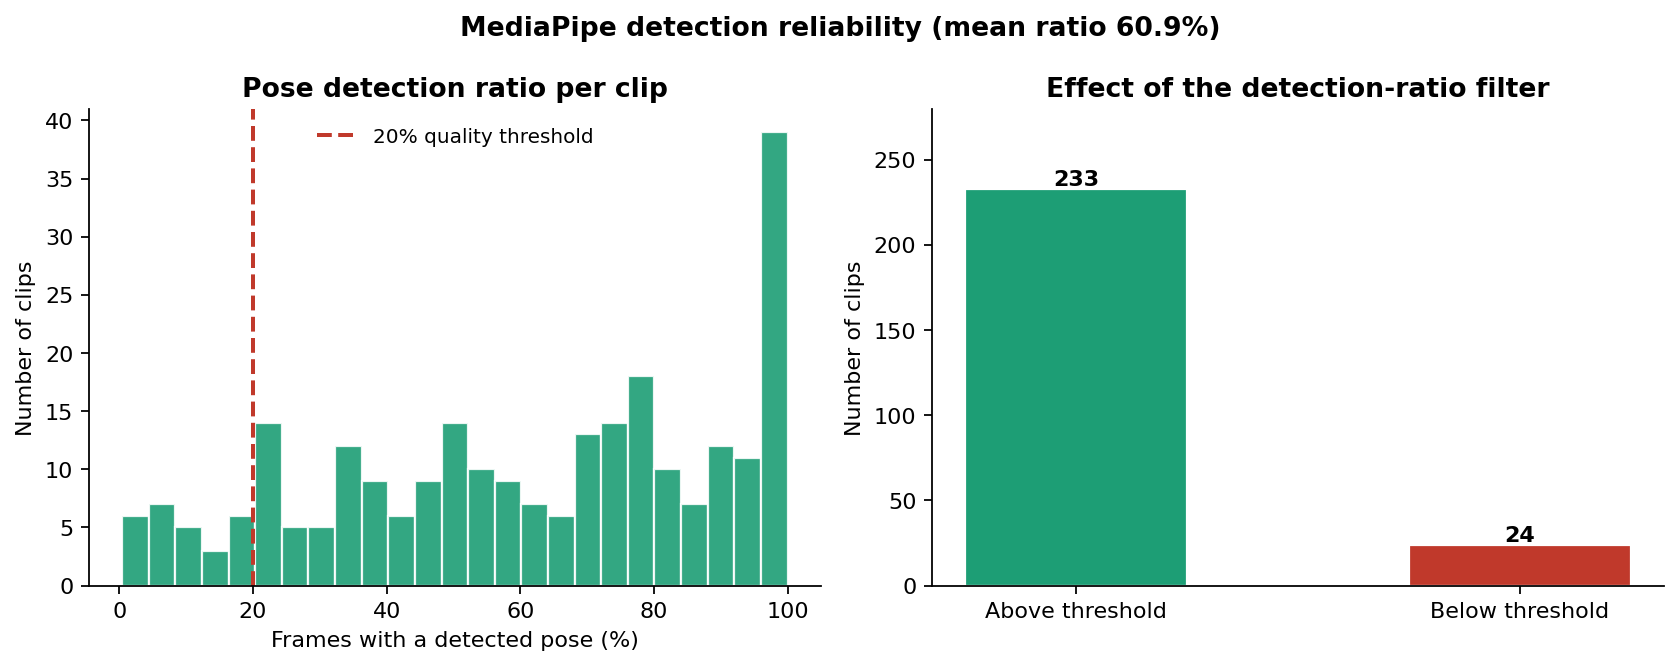
\includegraphics[width=0.99\textwidth]{fig14_detection_ratio.png}
    \caption{Pose detection ratio per clip and the effect of the 20 percent quality threshold}
    \label{fig:detection}
\end{figure}

\noindent
\textbf{Description:} Across 257 clips with a saved keypoint array, MediaPipe detected a pose in 60.9 percent of extracted frames on average, with a median of 66.0 percent. Thirty clips reached 100 percent detection and 24 clips fell below the 20 percent threshold and were therefore rejected. The distribution is broad rather than concentrated, which is itself the finding: pose extraction on this corpus is neither reliably successful nor reliably unsuccessful, but strongly dependent on how each individual clip was filmed.

Splitting the detection ratio by source makes the dependency explicit and quantifies the observation from the qualitative montage. Across the 61 locally recorded clips the mean detection ratio is 87.8 percent. Across the 195 broadcast clips it is 52.7 percent. The gap of thirty five percentage points is not a marginal effect, and it has a direct practical implication for the project: the cheapest available route to a larger and cleaner dataset is to record more footage locally rather than to source more broadcast penalties, because broadcast clips are both harder to obtain and roughly forty percent less likely to yield a usable pose stream per frame. This is why expanding the recorded corpus appears in the future work of Chapter 5.

\begin{figure}[H]
    \centering
    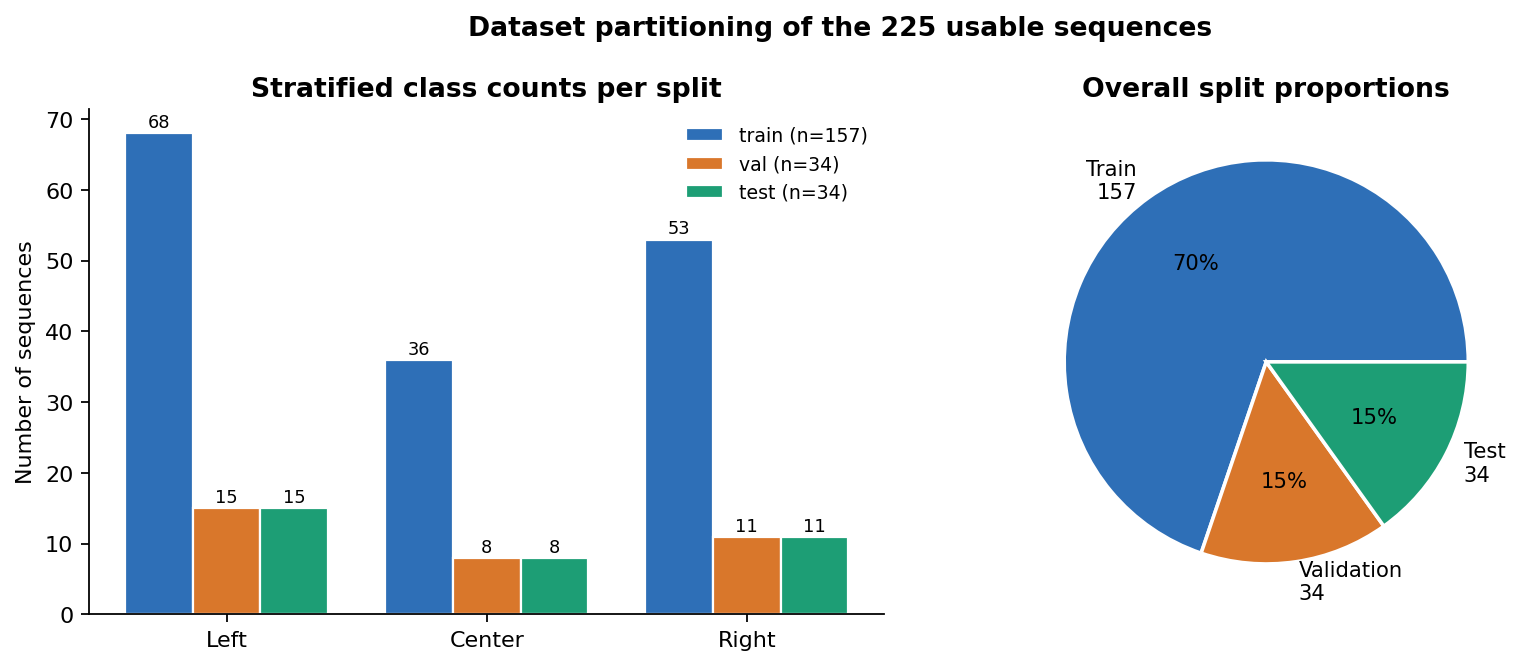
\includegraphics[width=0.99\textwidth]{fig15_split_distribution.png}
    \caption{Stratified partitioning of the 225 usable sequences}
    \label{fig:split}
\end{figure}

\noindent
\textbf{Description:} The stratified split preserves the class proportions in every partition. The training partition contains 68 left, 36 centre and 53 right sequences, and the validation and test partitions each contain 15 left, 8 centre and 11 right. The important consequence, and a limitation that must be kept in mind when reading every result in this chapter, is that with 34 test examples a single reclassified clip moves the reported accuracy by 2.9 percentage points. Differences smaller than about three points between configurations are therefore not meaningful, and this is stated here rather than glossed over because it governs how the ablation results should be interpreted.

\section{Quantitative Experiments}

\subsection{Evaluation Metrics and How They Are Validated}

The evaluation protocol is designed so that no information from the test partition influences the model in any way. The test set of 34 sequences is held out at the splitting stage, before any training occurs, and it is not used for early stopping, for checkpoint selection or for any hyperparameter decision. Early stopping monitors validation direction accuracy and restores the weights of the best validation epoch, so the validation set is consumed by model selection and its accuracy is consequently optimistic. The test accuracy is measured exactly once per configuration on the restored checkpoint. This separation is why the validation and test figures reported below differ, and why only the test figures should be read as estimates of generalisation.

\renewcommand{\arraystretch}{1.25}
\small
\begin{longtable}{|>{\bfseries}p{3.0cm}|p{4.4cm}|p{6.2cm}|}
\hline
\textbf{Metric} & \textbf{Definition} & \textbf{Why it is used here} \\ \hline
\endfirsthead
\hline
\textbf{Metric} & \textbf{Definition} & \textbf{Why it is used here} \\ \hline
\endhead
\hline
\multicolumn{3}{r}{\textit{Continued on next page}} \\
\hline
\endfoot
\hline
\endlastfoot
Accuracy & Correct predictions divided by total predictions & Primary headline metric, directly interpretable against the 33.3 percent random baseline \\ \hline
Precision & True positives over predicted positives, per class and weighted & Reveals whether a class is predicted too liberally \\ \hline
Recall & True positives over actual positives, per class and weighted & Reveals whether a class is being missed, which is the failure mode of the minority class \\ \hline
F1-score & Harmonic mean of precision and recall & Single summary per class that neither precision nor recall gives alone \\ \hline
Confusion matrix & Full three by three table of actual against predicted & Shows which specific classes are confused with which, not merely how often \\ \hline
MAE & Mean absolute error of the power prediction & Directly interpretable as an average error in points on the one to ten scale \\ \hline
MSE and RMSE & Mean squared error and its root & Penalise large power errors more heavily than MAE, exposing outliers \\ \hline
\caption{Evaluation metrics used and the reason each is reported}
\label{tab:metrics}
\end{longtable}
\normalsize

\noindent
\textbf{Description:} All classification metrics are computed with scikit-learn using weighted averaging for the aggregate figures, so that each class contributes in proportion to its support, and with division by zero handled explicitly so that an unpredicted class produces a score of zero rather than an undefined value. The weighted average is preferred over the macro average here because the class imbalance is a genuine property of the sport rather than a sampling artefact, so a metric that reflects the real class proportions is the more honest summary.

It is worth stating why these particular metrics are used rather than those a segmentation task would report. Mean intersection over union, the standard metric for semantic segmentation, measures the spatial overlap between a predicted region and a ground truth region. KickSense produces no spatial region: its direction output is a categorical choice among three classes and its power output is a scalar. There is nothing to intersect, so the intersection over union family is not merely unnecessary here but undefined. The classification and regression metrics above are the correct analogues, and the confusion matrix plays the diagnostic role for this task that a per class intersection over union table plays for segmentation.

\subsection{Reference Model Results}

All test set numbers in this subsection come from a single checkpoint, namely the full configuration trained with a fixed seed of forty two, which stopped at epoch 28 after early stopping restored the weights from its best validation epoch. Using one checkpoint for all of them ensures the confusion matrix, the per class metrics and the power regression plots describe the same model rather than a mixture of runs.

\begin{figure}[H]
    \centering
    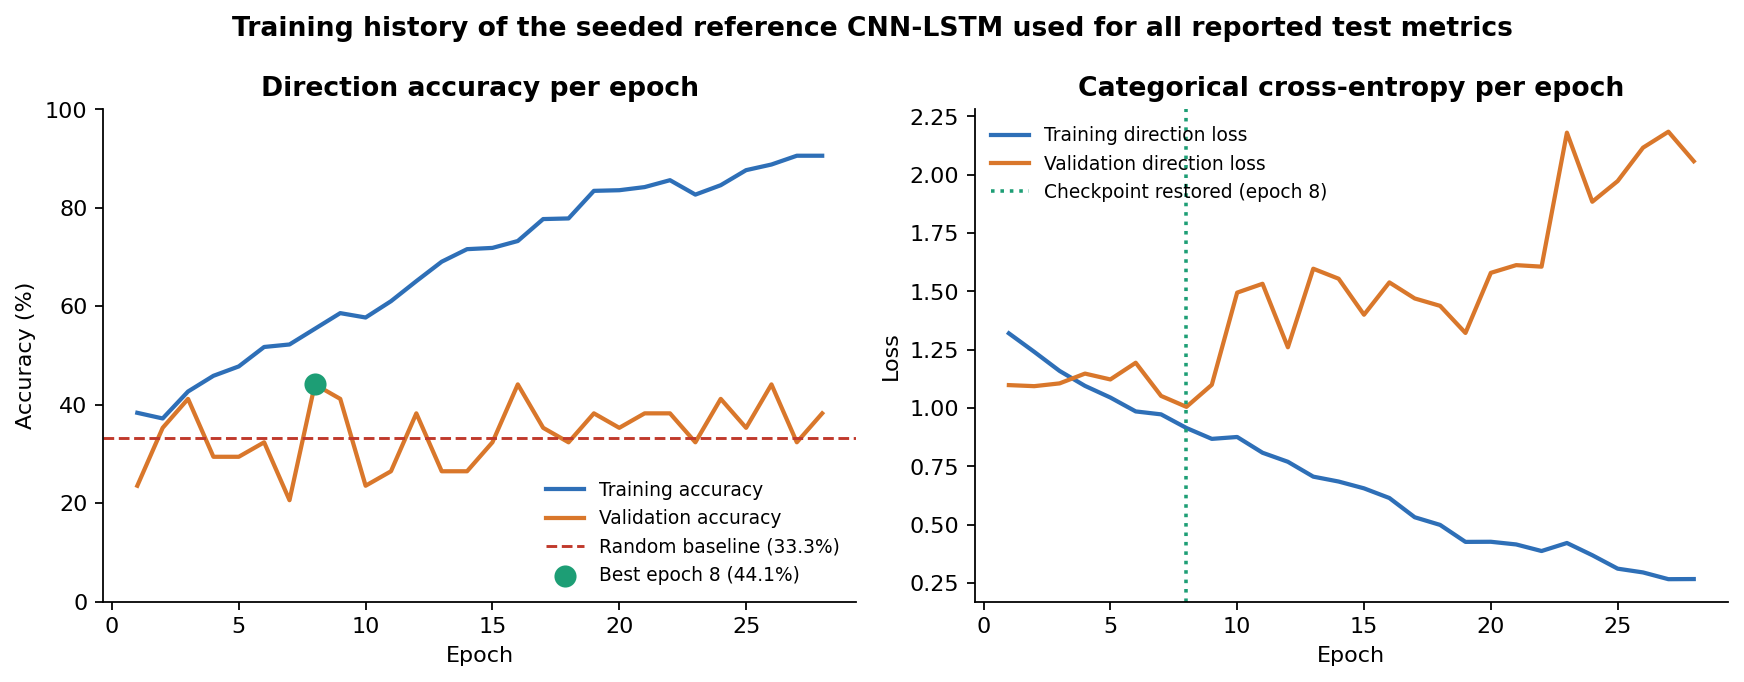
\includegraphics[width=0.99\textwidth]{fig18_training_curves.png}
    \caption{Training history of the seeded reference model}
    \label{fig:training}
\end{figure}

\noindent
\textbf{Description:} The left panel shows that training accuracy rises steadily and passes eighty percent while validation accuracy plateaus in the mid forties, which is the signature of overfitting on a small dataset and is precisely what the regularisation stack is intended to slow rather than eliminate. The right panel shows the corresponding cross entropy curves, with the validation loss flattening while the training loss continues to fall. Early stopping halts training at epoch 28 and restores the best validation epoch, so the divergence visible at the right hand edge of both panels is observed but not inherited by the evaluated model.

\renewcommand{\arraystretch}{1.3}
\small
\begin{longtable}{|>{\bfseries}p{6.0cm}|p{3.4cm}|p{4.0cm}|}
\hline
\textbf{Result} & \textbf{Value} & \textbf{Reference point} \\ \hline
\endfirsthead
\hline
\textbf{Result} & \textbf{Value} & \textbf{Reference point} \\ \hline
\endhead
\hline
\multicolumn{3}{r}{\textit{Continued on next page}} \\
\hline
\endfoot
\hline
\endlastfoot
Test set size & 34 sequences & 15 left, 8 centre, 11 right \\ \hline
Direction accuracy & 44.1 percent & Random baseline 33.3 percent \\ \hline
Weighted precision & 50.0 percent & \\ \hline
Weighted recall & 44.1 percent & Equal to accuracy by definition \\ \hline
Weighted F1-score & 41.4 percent & \\ \hline
Best validation accuracy, this run & 44.1 percent & Reached at epoch 8 \\ \hline
Best validation accuracy, any run & 55.9 percent & Epoch 29 of the visual label run \\ \hline
Best test accuracy, any logged run & 48.0 percent & Recorded in the first retrain log \\ \hline
Power MAE & 2.99 points & On the 1 to 10 scale \\ \hline
Power RMSE & 3.38 points & \\ \hline
Epochs to early stop & 28 & Patience 20 on validation accuracy \\ \hline
Trainable parameters & 248,580 & 249,220 including BN statistics \\ \hline
Augmented training sequences & 785 & From 157 originals \\ \hline
\caption{Quantitative results of the reference model on the held out test set}
\label{tab:test-results}
\end{longtable}
\normalsize

\noindent
\textbf{Description:} The headline result is 44.1 percent test direction accuracy against a 33.3 percent random baseline, which is a relative improvement of roughly a third over chance. Three separate accuracy figures are reported deliberately rather than only the most flattering one. The 44.1 percent is the reproducible test accuracy of the seeded reference model and is the figure that should be quoted as the current result. The 55.9 percent is the highest validation accuracy recorded anywhere in the project and is reported because it is a real measurement, but it is a validation figure and therefore optimistic. The 48.0 percent is the highest test accuracy recorded in any saved log. The spread between these numbers is itself a finding, discussed in Section 4.8.

\begin{figure}[H]
    \centering
    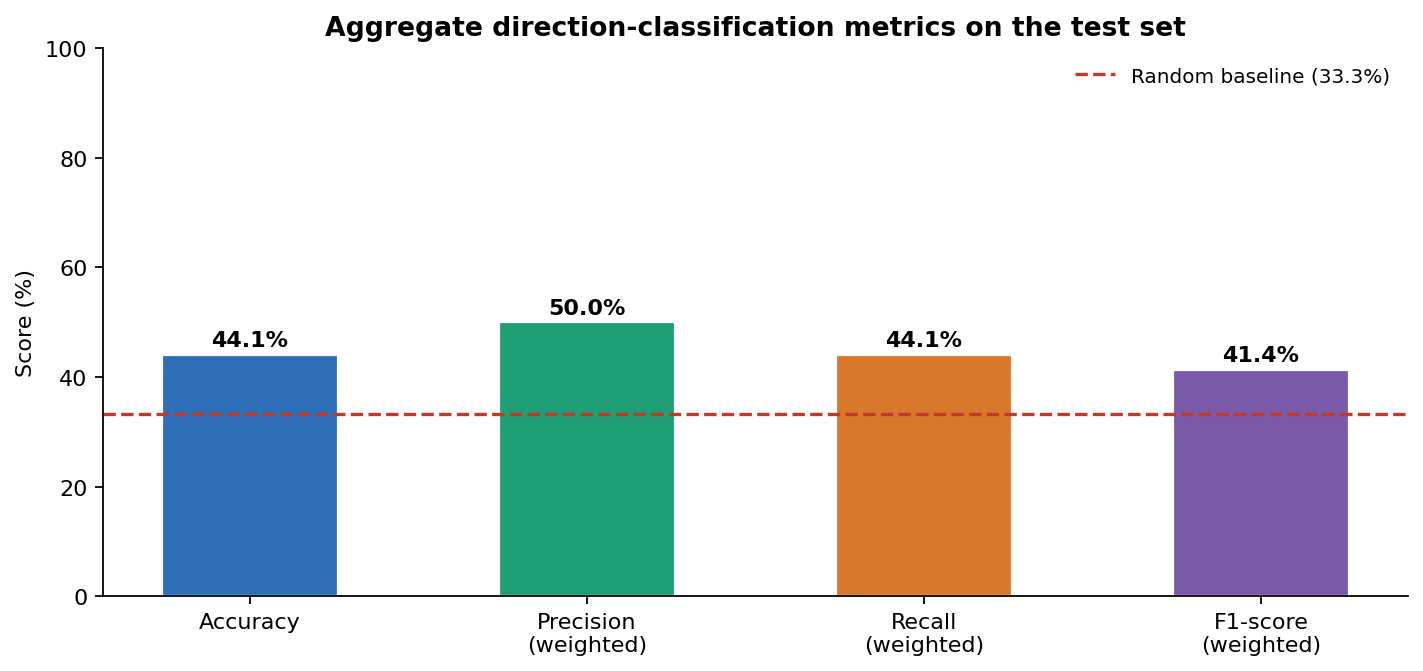
\includegraphics[width=0.99\textwidth]{fig21_metrics_overview.png}
    \caption{Aggregate direction classification metrics against the random baseline}
    \label{fig:metrics}
\end{figure}

\noindent
\textbf{Description:} All four aggregate metrics sit clearly above the 33.3 percent random baseline, which establishes that the model has learned a genuine signal rather than a class prior. The weighted precision of 50.0 percent exceeds the recall of 44.1 percent, which indicates the model is conservative in a specific way: when it commits to a class it is right half the time, but it fails to recover a majority of the true instances of at least one class. The confusion matrix identifies which.

\begin{figure}[H]
    \centering
    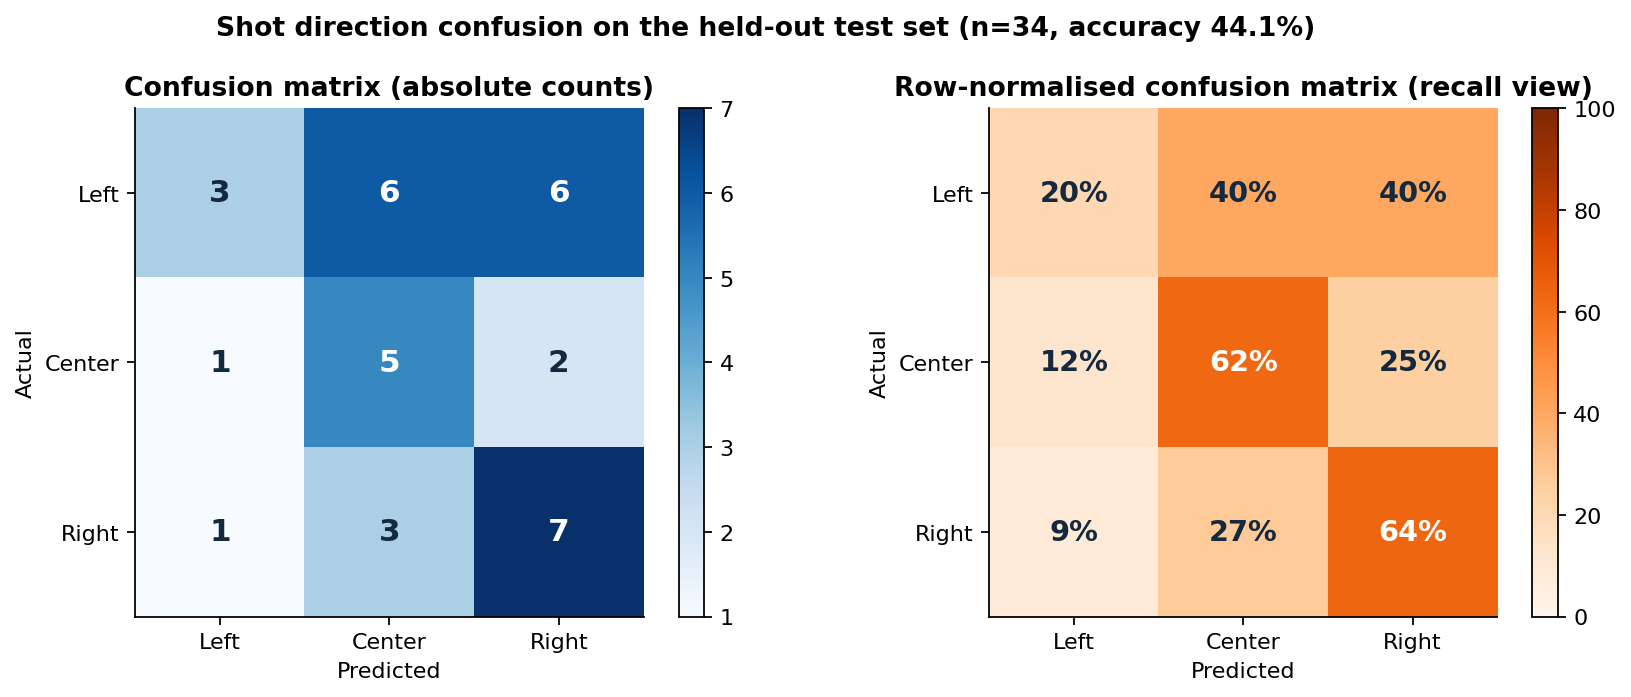
\includegraphics[width=0.99\textwidth]{fig19_confusion_matrix.png}
    \caption{Confusion matrix on the held out test set, in absolute counts and row normalised form}
    \label{fig:confusion}
\end{figure}

\noindent
\textbf{Description:} The confusion matrix is the most diagnostic result in the chapter. Reading the rows, the left class is recovered in only 3 of 15 cases, with 6 misclassified as centre and 6 as right. The centre class is recovered in 5 of 8 cases and the right class in 7 of 11. The pattern is therefore not a uniform difficulty but a specific and asymmetric failure: the model systematically under predicts left shots and disperses them across the other two classes, while handling right and centre comparatively well. This is a more useful finding than the accuracy figure alone, because it points at a concrete cause. The mirror augmentation converts every left example into a right example and vice versa, so after augmentation the left and right classes are numerically balanced; if the underlying left examples are visually harder, for instance because more of them come from broadcast clips filmed from an angle that foreshortens the run up, then balance in count does not translate into balance in learnability. Investigating this asymmetry is a concrete next step rather than a general aspiration.

\begin{figure}[H]
    \centering
    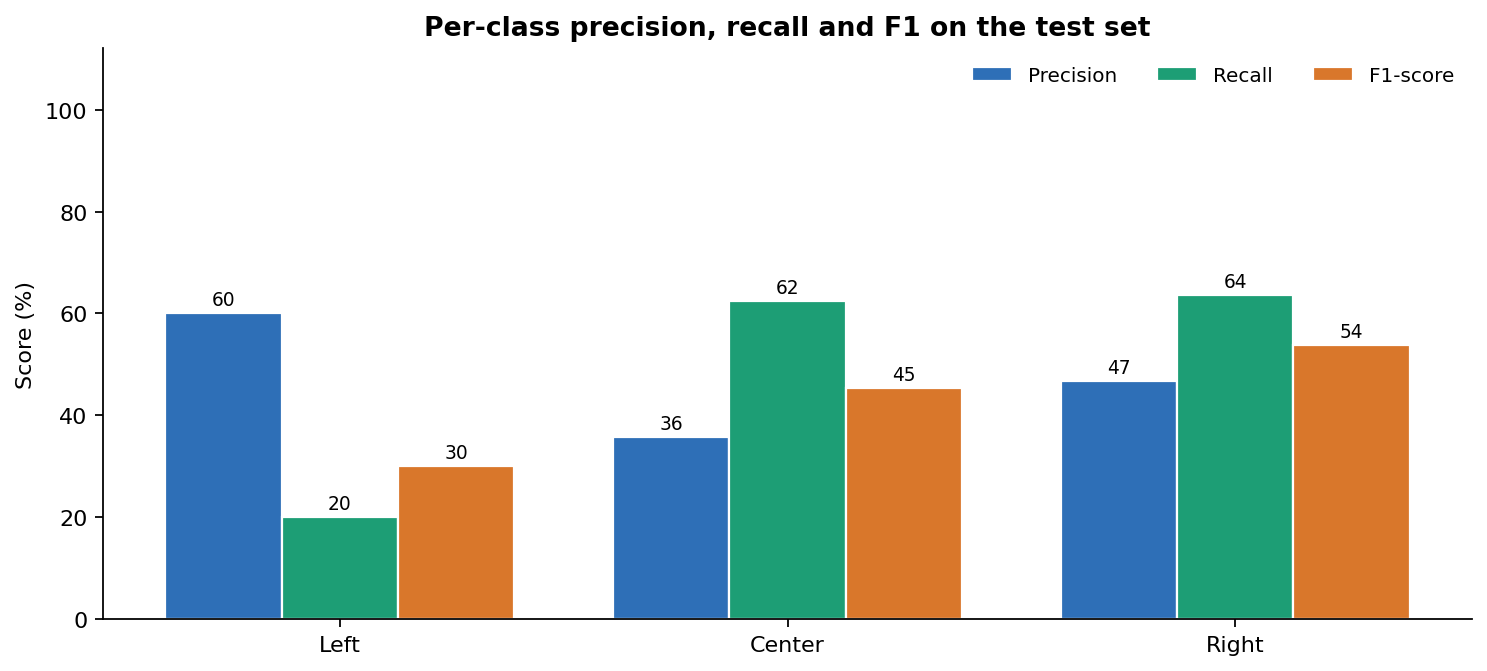
\includegraphics[width=0.92\textwidth]{fig20_per_class_metrics.png}
    \caption{Per class precision, recall and F1 score on the test set}
    \label{fig:per-class}
\end{figure}

\noindent
\textbf{Description:} The per class breakdown quantifies the asymmetry the confusion matrix exposes. The left class attains 60.0 percent precision but only 20.0 percent recall, giving an F1 of 30.0 percent, which is the profile of a class the model predicts rarely but with reasonable reliability when it does. The centre class attains 35.7 percent precision with 62.5 percent recall and an F1 of 45.5 percent, the opposite profile of a class the model over predicts. The right class is the most balanced at 46.7 percent precision, 63.6 percent recall and 53.8 percent F1. Notably, the centre class is not the weakest despite having the least support, which suggests the class weighting is doing its job and that support alone does not determine per class performance here.

\begin{figure}[H]
    \centering
    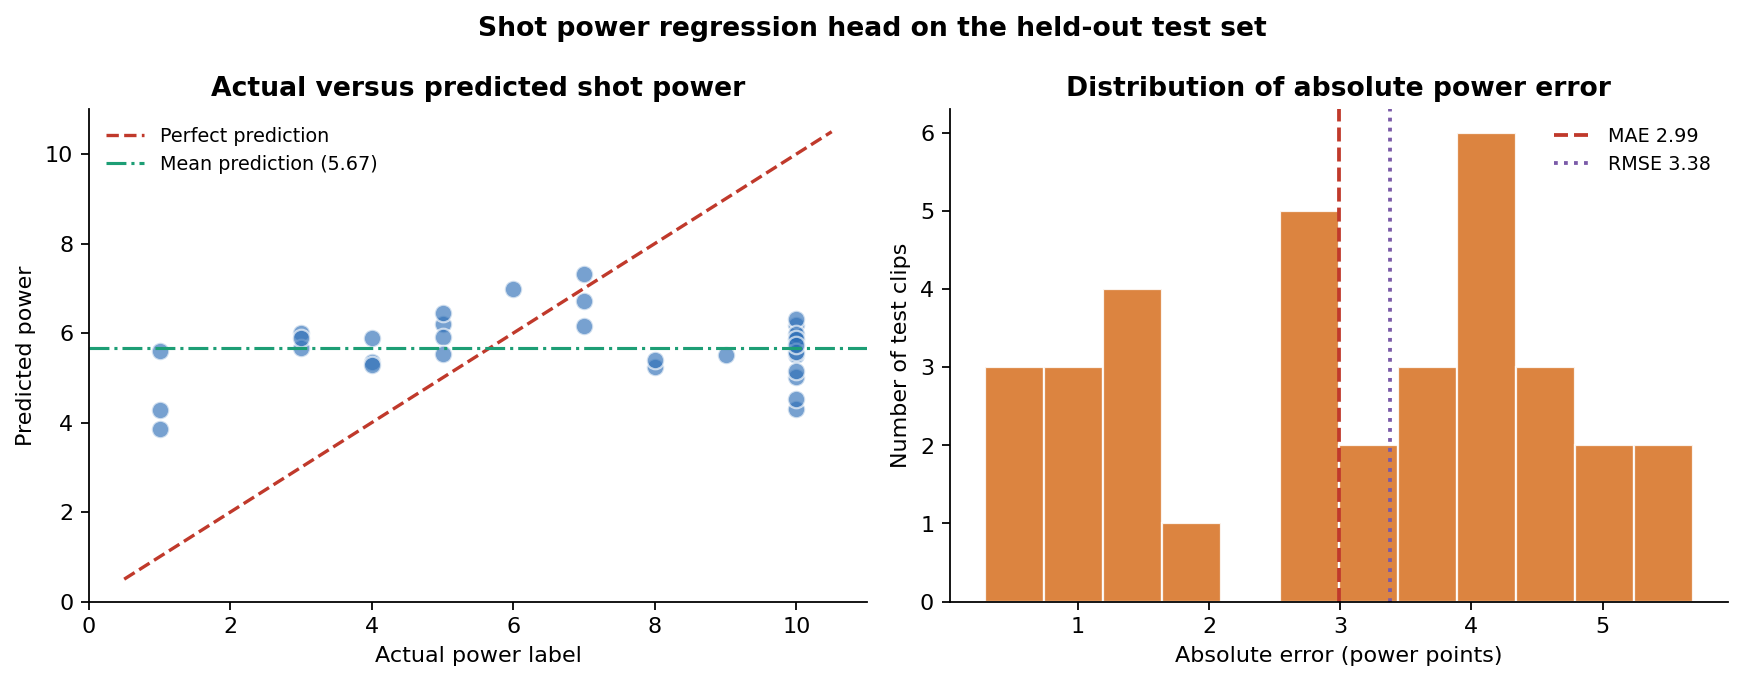
\includegraphics[width=0.99\textwidth]{fig22_power_regression.png}
    \caption{Shot power regression behaviour on the test set}
    \label{fig:power-reg}
\end{figure}

\noindent
\textbf{Description:} The power head performs poorly, and the left panel shows why in a way the error metric alone does not. The predictions cluster in a narrow horizontal band rather than following the diagonal, which means the model is largely predicting a value close to the training mean regardless of the input. The mean absolute error of 2.99 points on a one to ten scale should therefore be read as evidence that the power head has not learned a useful mapping rather than as evidence of moderate accuracy. The cause is diagnosable from Section 4.2: the power labels are strongly bimodal with 76 clips at ten and 40 at one, so the target is closer to a coarse category than a graded measurement, and predicting the mean is close to the optimal strategy under mean squared error for a target the input cannot explain. Replacing the subjective scale with a measurement derived from frame to frame ball displacement is consequently the highest value item in the future work of Chapter 5, and the honest statement of the current position is that direction prediction works above chance while power prediction does not yet work.

\section{Ablation Study}

The ablation study trains six configurations under identical conditions with the same seed and the same split, each differing from the full model by exactly one factor. Its purpose is to determine which design decisions contribute to the result, which is a question the development history cannot answer because those runs differed in several respects at once.

\begin{figure}[H]
    \centering
    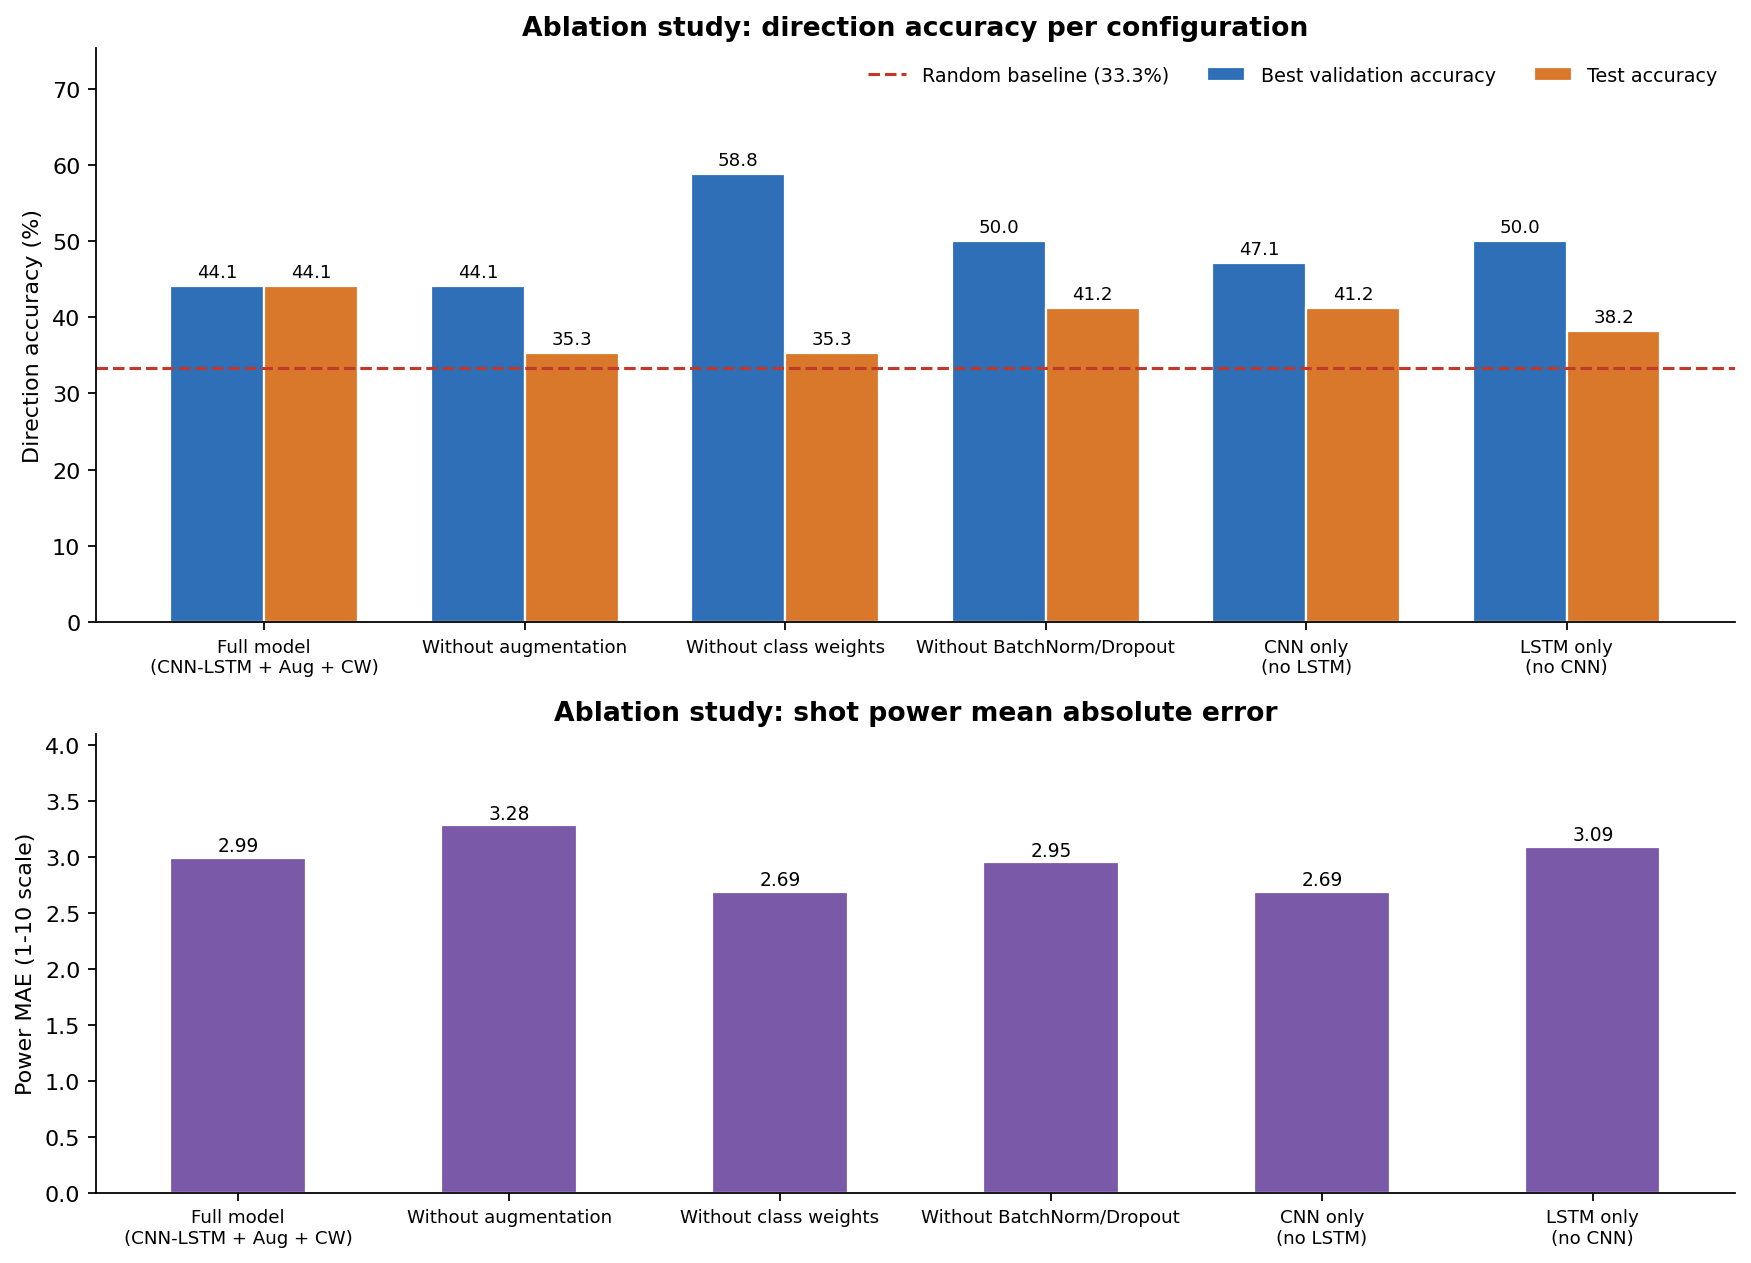
\includegraphics[width=0.99\textwidth]{fig23_ablation_study.png}
    \caption{Ablation study over architecture, augmentation, class weighting and regularisation}
    \label{fig:ablation}
\end{figure}

\noindent
\textbf{Description:} The upper panel reports the best validation accuracy and the test accuracy of each configuration and the lower panel reports the power mean absolute error. The full model attains the highest test accuracy of all six configurations, and every ablated variant is worse on the test set, which supports the architecture as a whole. The validation figures do not rank the configurations in the same order as the test figures, which is discussed below and is a finding in its own right.

\begin{table}[H]
\centering
\renewcommand{\arraystretch}{1.3}
\setlength{\tabcolsep}{4pt}
\small
\begin{tabular}{|>{\raggedright\arraybackslash\bfseries}p{4.0cm}|r|r|r|r|r|}
\hline
\textbf{Configuration} & \textbf{Params} & \textbf{Epochs} & \textbf{Val. acc.} & \textbf{Test acc.} & \textbf{MAE} \\ \hline
Full model (CNN-LSTM, augmentation, class weights) & 249,220 & 28 & 44.1\% & \textbf{44.1\%} & 2.99 \\ \hline
Without augmentation & 249,220 & 21 & 44.1\% & 35.3\% & 3.28 \\ \hline
Without class weights & 249,220 & 63 & \textbf{58.8\%} & 35.3\% & \textbf{2.69} \\ \hline
Without BatchNorm and Dropout & 247,940 & 35 & 50.0\% & 41.2\% & 2.95 \\ \hline
CNN only, no LSTM & 76,420 & 46 & 47.1\% & 41.2\% & 2.69 \\ \hline
LSTM only, no CNN & 200,388 & 46 & 50.0\% & 38.2\% & 3.09 \\ \hline
Random baseline & n/a & n/a & 33.3\% & 33.3\% & n/a \\ \hline
\end{tabular}
\caption{Ablation results, all configurations trained with seed 42 on the identical split}
\label{tab:ablation}
\end{table}
\normalsize
\setlength{\tabcolsep}{6pt}

\noindent
\textbf{Description:} Reading the test accuracy column, the full model at 44.1 percent leads, followed by the two variants at 41.2 percent, the recurrent only variant at 38.2 percent, and the two weakest at 35.3 percent. The power mean absolute error column shows much less variation, between 2.69 and 3.28, which is consistent with the finding of Section 4.6 that no configuration has learned a useful power mapping.

Four conclusions follow, and they are stated with the precision the test set size permits.

The clearest result is that \textbf{augmentation matters}. Removing it drops test accuracy from 44.1 to 35.3 percent, a gap of 8.8 percentage points corresponding to three test clips, and it also produces the worst power error of any configuration at 3.28. It additionally stops training earliest, at 21 epochs, which is the expected consequence of training on 157 rather than 785 sequences. This is the only individual effect in the table large enough to sit comfortably outside the roughly three point noise floor established in Section 4.5.

The second result is that \textbf{both halves of the encoder contribute}. Removing the recurrent layers costs 2.9 points of test accuracy and removing the convolutional layers costs 5.9 points, so neither component is redundant and the hybrid outperforms either alone. The convolution only variant is the more interesting of the two, because it reaches 41.2 percent with 76,420 parameters, less than a third of the full model. Given the dataset size this is worth noting explicitly: a substantially smaller model is nearly as accurate, which suggests the full model's capacity is not the limiting factor and that data, not architecture, is the binding constraint.

The third result concerns \textbf{class weighting}, and it is the most instructive because it is counterintuitive. Removing class weighting produces the highest validation accuracy in the entire table, at 58.8 percent, while simultaneously producing one of the lowest test accuracies, at 35.3 percent. Two things follow. First, this configuration is the one that matches the production training script, since as noted in Chapter 3 that script computes class weights but cannot pass them to a multi output Keras model, which explains why the 55.9 percent validation figure recorded in the project logs is consistent with the 58.8 percent observed here. Second, and more importantly, a 23 point gap between validation and test accuracy in the same run demonstrates that with 34 validation examples the validation set is too small to select models reliably. This is a genuine methodological weakness of the current protocol and it is the reason that stratified k fold cross validation, rather than a single held out validation split, is listed as future work.

The fourth result is that \textbf{removing regularisation is not catastrophic}, costing 2.9 points of test accuracy, which is within the noise floor. The regularisation stack should therefore be understood as a reasonable precaution whose benefit is not individually measurable at this dataset size rather than as a demonstrated necessity.

\section{Development History}

\begin{figure}[H]
    \centering
    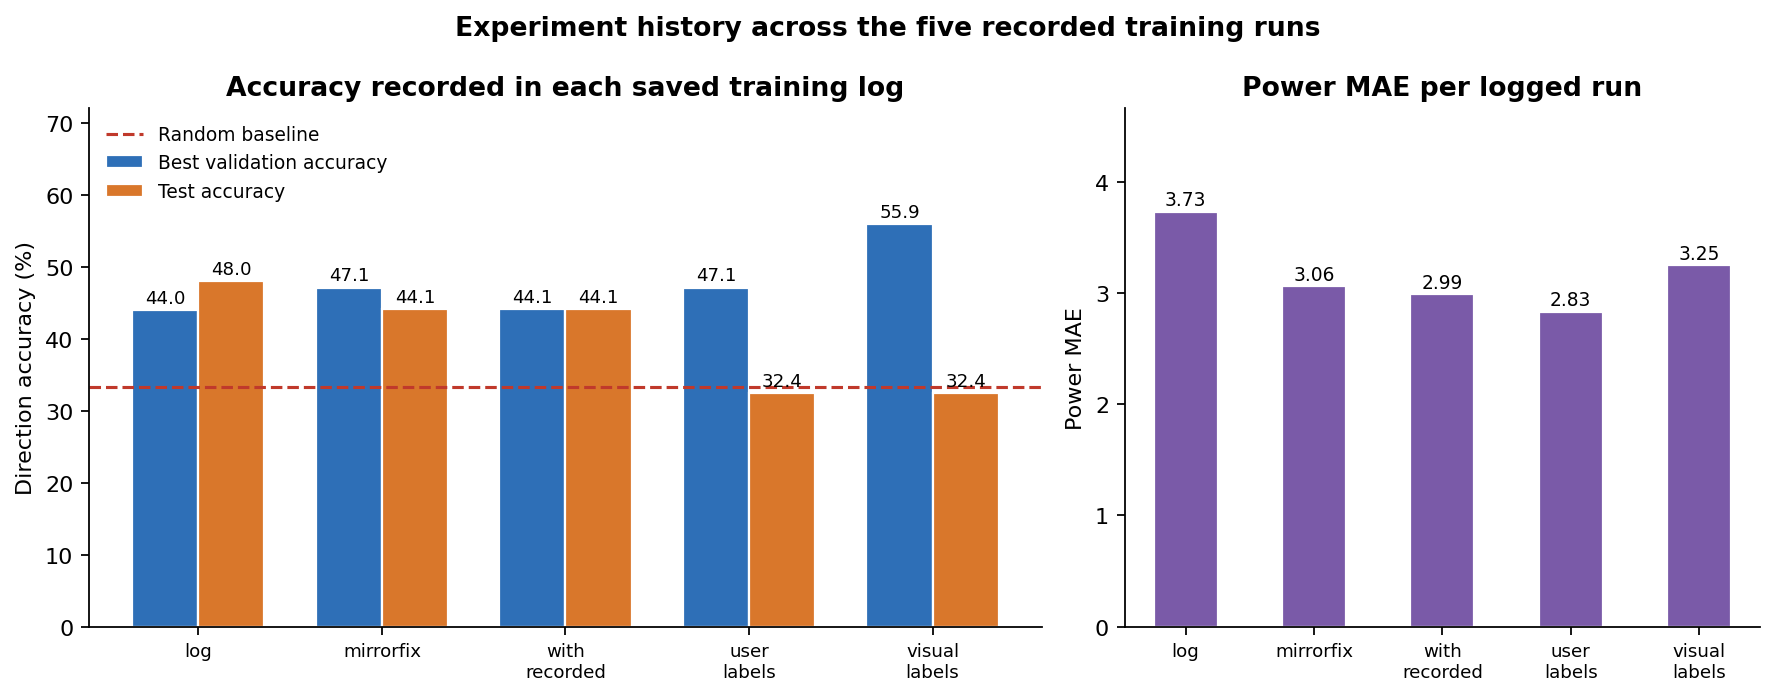
\includegraphics[width=0.99\textwidth]{fig24_run_comparison.png}
    \caption{Accuracy and power error recorded across the five saved training runs}
    \label{fig:runs}
\end{figure}

\noindent
\textbf{Description:} These five runs are the preserved development history, and unlike the ablation they differ from one another in the state of the data as well as the code, so they document progress rather than support attribution. Validation accuracy improves across the sequence from 44.0 to 55.9 percent as the corpus grew with locally recorded footage, a defect in the mirror augmentation was corrected, and a portion of the direction labels was re-verified against the video. Test accuracy does not follow the same trend, which is the same instability the ablation exposed.

\begin{figure}[H]
    \centering
    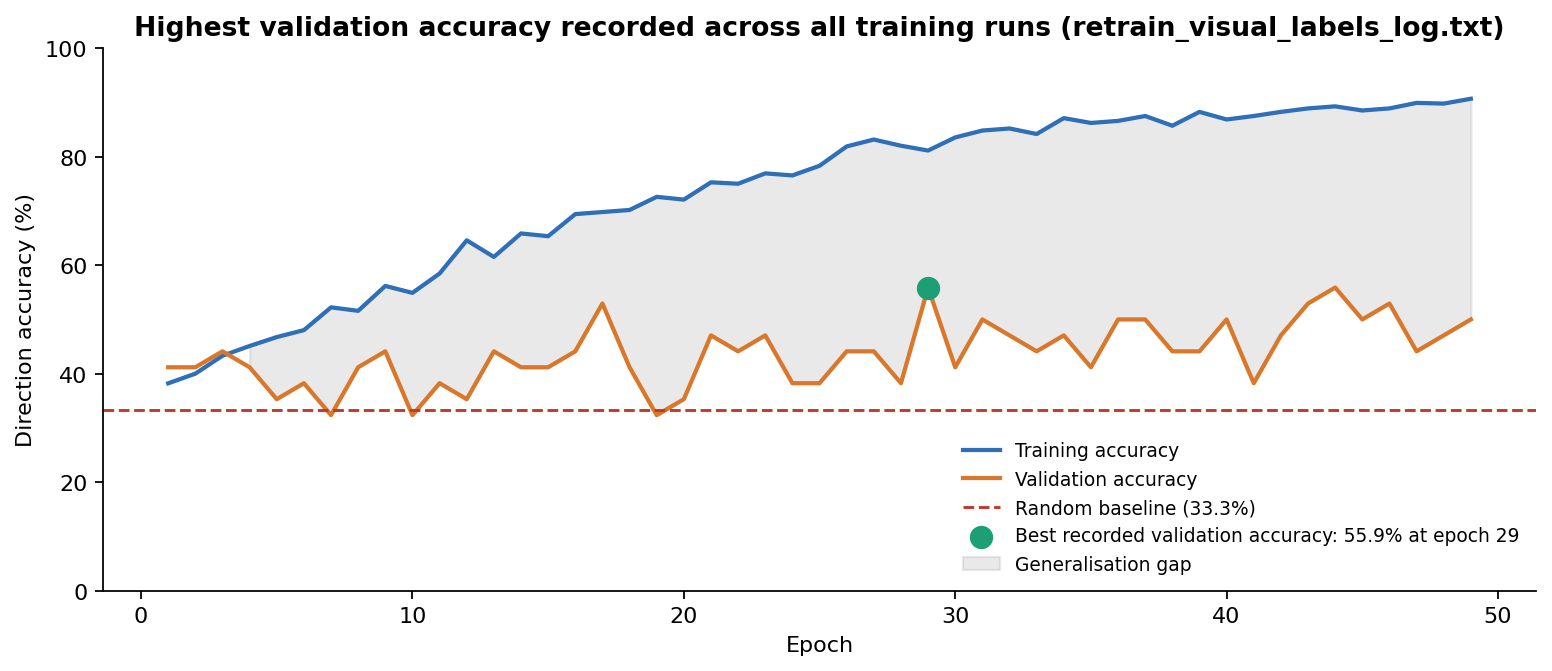
\includegraphics[width=0.99\textwidth]{fig28_historical_best_run.png}
    \caption{The training run that produced the highest validation accuracy recorded in the project}
    \label{fig:historical}
\end{figure}

\noindent
\textbf{Description:} This figure shows the full 49 epoch history of the run that reached 55.9 percent validation direction accuracy at epoch 29, the highest figure recorded anywhere in the project. The shaded region marks the generalisation gap between training and validation accuracy, which widens steadily as training progresses and is the visual signature of the small dataset problem. The run is presented here because it is a genuine logged measurement, but the reference model of Section 4.6 rather than this run is the basis for every test set number in this chapter, because this checkpoint was subsequently overwritten by later retraining and cannot be re-evaluated.

\begin{table}[H]
\centering
\renewcommand{\arraystretch}{1.3}
\setlength{\tabcolsep}{4pt}
\small
\begin{tabular}{|>{\raggedright\arraybackslash\bfseries}p{3.4cm}|r|r|r|>{\raggedright\arraybackslash}p{4.0cm}|}
\hline
\textbf{Saved log} & \textbf{Val. acc.} & \textbf{Test acc.} & \textbf{MAE} & \textbf{Change in that run} \\ \hline
retrain & 44.0\% & 48.0\% & 3.73 & Baseline, 114 training samples \\ \hline
with\_recorded & 44.1\% & 44.1\% & 2.99 & Locally recorded clips added \\ \hline
mirrorfix & 47.1\% & 44.1\% & 3.06 & Mirror augmentation defect corrected \\ \hline
user\_labels & 47.1\% & 32.4\% & 2.83 & Direction labels revised \\ \hline
visual\_labels & \textbf{55.9\%} & 32.4\% & 3.25 & Labels re-verified against footage \\ \hline
\end{tabular}
\caption{The five recorded training runs and the change introduced in each. Log file names are abbreviated from \texttt{retrain\_*\_log.txt} in \texttt{outputs/model}}
\label{tab:run-history}
\end{table}
\normalsize
\setlength{\tabcolsep}{6pt}

\noindent
\textbf{Description:} This table records the development history honestly, including the fact that the two runs with the highest validation accuracy have the lowest test accuracy. Presented alone either column would be misleading. Presented together they show that improvements which appeared real when measured on 34 validation examples did not transfer to the test partition, and this is the single strongest piece of evidence that the evaluation protocol, rather than the model, is the immediate bottleneck in the project.

\section{Comparison with the Base Paper}

The base paper of Salazar and Alatrista-Salas addresses the same prediction task with the same three way regional formulation \cite{salazar2024}, so a comparison is natural. It is nonetheless not possible to make a numerical one, and the reason must be stated plainly rather than worked around. Both projects had to construct a bespoke corpus because no public dataset annotates penalty direction, and the base paper's corpus is not publicly released. The two datasets therefore differ in size, in the competitions they draw from, in camera angles, and in annotation schema. An accuracy figure obtained on one corpus and an accuracy figure obtained on the other measure the difficulty of two different datasets at least as much as they measure the quality of two different models, so placing them side by side and declaring a winner would be a claim the evidence cannot support. No such claim is made in this report.

What can be compared is methodology, computational cost, output scope and evaluation rigour, and Table \ref{tab:metric-compare} does so.

\renewcommand{\arraystretch}{1.3}
\small
\begin{longtable}{|>{\raggedright\arraybackslash\bfseries}p{3.4cm}|>{\raggedright\arraybackslash}p{4.9cm}|>{\raggedright\arraybackslash}p{4.9cm}|}
\hline
\textbf{Aspect} & \textbf{Salazar and Alatrista-Salas (2024)} & \textbf{KickSense} \\ \hline
\endfirsthead
\hline
\textbf{Aspect} & \textbf{Salazar and Alatrista-Salas (2024)} & \textbf{KickSense} \\ \hline
\endhead
\hline
\multicolumn{3}{r}{\textit{Continued on next page}} \\
\hline
\endfoot
\hline
\endlastfoot
Evaluation dataset & Bespoke corpus, not publicly released & Bespoke corpus of 225 usable sequences, fully documented in this repository \\ \hline
Metrics reported & Accuracy of regional prediction, plus a study of body part influence & Accuracy, weighted and per class precision, recall and F1, confusion matrix, MAE, MSE and RMSE \\ \hline
Reason the metrics differ & Single classification output, so accuracy plus interpretability analysis suffices & Two heads require both classification and regression metrics; per class metrics are necessary because the classes are unbalanced \\ \hline
Random baseline stated & Not emphasised & Stated explicitly as 33.3 percent alongside every accuracy figure \\ \hline
Test protocol & Not fully specified in the published description & Held out 34 sequence test split, never used for early stopping or model selection, evaluated once per configuration \\ \hline
Pose stage cost & TAM segmentation and MMPose 3D pose, requires a graphics processor & MediaPipe Pose on CPU, runs on a consumer laptop \\ \hline
Output scope & Goal region only & Goal region plus a shot power estimate \\ \hline
Ablation analysis & Three model families compared & Six configurations varying architecture, augmentation, class weighting and regularisation, all under one seed and split \\ \hline
Direct accuracy comparison & \multicolumn{2}{|>{\raggedright\arraybackslash}p{10.3cm}|}{Not performed. The corpora differ and neither is available to the other, so any head to head accuracy claim would be unsupported.} \\ \hline
\caption{Comparison of the evaluation protocols of the base paper and KickSense}
\label{tab:metric-compare}
\end{longtable}
\normalsize

\noindent
\textbf{Description:} The comparison is deliberately restricted to what the available evidence supports. KickSense reports a broader metric set on a documented and reproducible split, and it delivers an additional output that the base paper does not attempt, at a computational cost low enough for consumer hardware. It does not claim higher accuracy, because the datasets differ. The one point on which KickSense is unambiguously ahead is reproducibility, since every figure and every number in this chapter can be regenerated from the repository, which is not true of a result reported on an unreleased corpus.

\section{Summary of Findings}

The evaluation supports five conclusions. First, the direction prediction works above chance, at 44.1 percent test accuracy against a 33.3 percent baseline, and this is a real if modest result. Second, the power prediction does not yet work, since the head largely predicts the training mean, and the diagnosis points at the bimodal subjective annotation rather than at the architecture. Third, the pose stage is the dominant data quality bottleneck, with an average detection ratio of 87.8 percent on locally recorded clips against 52.7 percent on broadcast clips, which makes local recording the most efficient route to a better dataset. Fourth, augmentation is the only training component whose individual contribution is measurable above the noise floor, and both halves of the hybrid encoder contribute while a model a third of the size is nearly as accurate, which together indicate that data rather than model capacity is the binding constraint. Fifth, and most consequentially for the next phase of the project, a 34 example validation set is too small for reliable model selection, as demonstrated by a 23 point validation to test gap within a single run, which makes cross validation the highest priority methodological fix.

\clearpage
